\documentclass[10pt]{article}
\usepackage[a4paper,top=2.8cm,bottom=2.8cm,left=2.3cm,right=2.3cm]{geometry}
\usepackage{xeCJK}
\usepackage{fontspec}
\usepackage{graphicx}
\usepackage{xcolor}
\usepackage{indentfirst}
\usepackage{tikz}
\usepackage{pgfplots}
\usepackage{amssymb}
\usepackage{amsthm}
\usepackage{amsmath}
\usepackage{fancyhdr}
\usepackage{tabularx}
\usepackage{hyperref}
\usepackage{xurl}
\usepackage{ulem}
\usepackage{version}
\usepackage{thmtools}
\usepackage{qtree}
\usepackage{algorithm}
\usepackage{algpseudocode}
\usepackage{mathtools}
\usepackage[shortlabels]{enumitem}
\usepackage{mdframed}
\usepackage{lipsum}
\usepackage{listings}

\XeTeXlinebreaklocale "zh"
\XeTeXlinebreakskip = 0pt plus 1pt

\setCJKmainfont{Noto Serif CJK TC}
\setmonofont{Source Code Pro}
\usetikzlibrary{arrows,decorations.markings,decorations.pathreplacing}
\pagestyle{fancy}

\tikzstyle {graph node} = [circle, draw, minimum width=1cm]
\tikzset{edge/.style = {decoration={markings,mark=at position 1 with %
            {\arrow[scale=2,>=stealth]{>}}},postaction={decorate}}}

\renewcommand{\baselinestretch}{1.3}

\newtheoremstyle{owo}% name of the style to be used
  {10pt}% measure of space to leave above the theorem. E.g.: 3pt
  {10pt}% measure of space to leave below the theorem. E.g.: 3pt
  {}% name of font to use in the body of the theorem
  {}% measure of space to indent
  {\bfseries}% name of head font
  { }% punctuation between head and body
  { }% space after theorem head; " " = normal interword space
  {\thmname{#1}\thmnumber{ #2}.\thmnote{ (#3)}}

\theoremstyle{owo}
\newtheorem{Theorem}{Theorem}
\newtheorem{Lemma}{Lemma}
\newtheorem{Observation}{Observation}
\newtheorem{Corollary}{Corollary}
\newtheorem*{Proof}{Proof}

\DeclareMathOperator*{\argmin}{argmin}

\hypersetup{
    %colorlinks=true,
    }

\newmdenv[topline=false, bottomline=false, rightline=false, linewidth=3pt, linecolor=black!10!white]{Quotemd}
\newenvironment{Quote}{~\vspace{-15pt}\begin{Quotemd}}{\end{Quotemd}}

\lstset{
    basicstyle=\ttfamily\footnotesize,
    numberstyle=\footnotesize,
    %numbers=left,
    stepnumber=1,
    numbersep=3pt,
    commentstyle=\color{black!50},
    keywordstyle=\color{white!0!blue},
    stringstyle=\color{black!50!green},
    showspaces=false,
    showstringspaces=false,
    showtabs=false,
    tabsize=4,
    captionpos=b,
    breaklines=true,
    breakatwhitespace=false,
    escapeinside={\%*}{*)},
    morekeywords={*}
}

\begin{document}

\renewcommand{\headrulewidth}{1pt}
\pagenumbering{arabic}
\setlength\parindent{20pt}
\setlength\parskip{10pt}
\cfoot{\thepage}
\lhead{Left}
\chead{Center}
\rhead{Right}

\setlist[enumerate]{itemsep=0pt, parsep=0pt, topsep=0pt}
\setlist[itemize]{itemsep=0pt, parsep=0pt, topsep=0pt}

\section*{Problem 1}

\subsection*{(a)}

孔乙己是站着喝酒而穿長衫的唯一的人。他身材很高大;青白臉色,皺紋間時常夾些傷痕;一部亂蓬蓬的花白的鬍子。穿的雖然是長衫,可是又髒又破,似乎十多年沒有補,也沒有洗。他對人說話,總是滿口之乎者也,教人半懂不懂的。因爲他姓孔,別人便從描紅紙上的「上大人孔乙己」這半懂不懂的話裏,替他取下一個綽號,叫作孔乙己。孔乙己一到店,所有喝酒的人便都看着他笑,有的叫道,「孔乙己,你臉上又添上新傷疤了!」他不回答,對櫃裏說,「溫兩碗酒,要一碟茴香豆。」便排出九文大錢。他們又故意的高聲嚷道,「你一定又偷了人家的東西了!」孔乙己睜大眼睛說,「你怎麼這樣憑空汚人清白……」「什麼清白?我前天親眼見你偷了何家的書,吊着打。」孔乙己便漲紅了臉,額上的青筋條條綻出,爭辯道,「竊書不能算偷……竊書!……讀書人的事,能算偷麼?」接連便是難懂的話,什麼「君子固窮」,什麼「者乎」之類,引得衆人都鬨笑起來:店內外充滿了快活的空氣。

Example for inline code: \texttt{hello}

\lipsum[1]

\begin{Lemma}
    \lipsum[2]
\end{Lemma}

\begin{Proof}
    \lipsum[3]
    \qed
\end{Proof}

\begin{Theorem}[Name]
    \lipsum[4]
\end{Theorem}

\begin{lstlisting}
hihihi
\end{lstlisting}

\lipsum[9]

\begin{lstlisting}[language=C++]
int main(){
    cout << "owo\n";
    return 0; // hello
}
\end{lstlisting}

\lipsum[10]

\begin{lstlisting}[language=Python]
for i in range(1, 100):
    print("123") # hello
\end{lstlisting}

\lipsum[11]

\begin{Quote}
    \lipsum[5]
\end{Quote}

\lipsum[6]
\begin{itemize}
    \item 1
    \item 2
\end{itemize}
\lipsum[7]
\begin{enumerate}
    \item 1
    \item 2
\end{enumerate}
\begin{enumerate}[(a)]
    \item 1
    \item 2
\end{enumerate}

\begin{figure}
    \begin{center}
        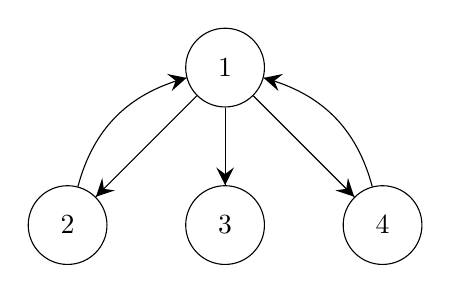
\begin{tikzpicture}
            \node[graph node] (v1) at (0, 0) {$1$};
            \node[graph node] (v2) at (-2, -2) {$2$};
            \node[graph node] (v3) at (0, -2) {$3$};
            \node[graph node] (v4) at (2, -2) {$4$};
            \draw[edge] (v1) -- (v2);
            \draw[edge] (v1) -- (v3);
            \draw[edge] (v1) -- (v4);
            \draw[edge] (v2) to [bend left] (v1);
            \draw[edge] (v4) to [bend right] (v1);
        \end{tikzpicture}
    \end{center}

    \caption{test}
\end{figure}

\begin{algorithm}
    \caption{hello}
    \begin{algorithmic}
        \State $i \gets 1$
        \ForAll{$j \in S$}
            \State $i \gets i + j$
        \EndFor
    \end{algorithmic}
\end{algorithm}

\end{document}
